\section{Objectives and Optimization Framework}
\label{sec:objectives}

Let $S$ be the set of accounts selected for review. Its size is the account budget. The original graph has $|M|=12{,}217$ accounts and $|R_{\text{wf}}|=7{,}171$ workflow-associated repository keys. For each account $m\in M$, $E_m\subseteq R_{\text{wf}}$ contains the repositories reachable from packages associated with $m$. For repository $r$, $\operatorname{Sources}(r)=\{m\in M:r\in E_m\}$ is its set of observed upstream sources.

Figure~\ref{fig:q1_methodology} summarizes the analysis and consistency checks.

\begin{figure}[t]
\centering
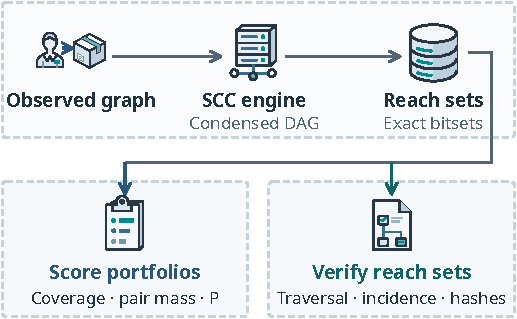
\includegraphics[width=\columnwidth]{study_methodology.pdf}
\caption{The observed graph yields exact reach sets through strongly connected component condensation and bitset unions. The sets supply both fixed-budget scoring and reachability checks. Comparisons use the same graph within each representation.}
\label{fig:q1_methodology}
\end{figure}

\subsection{Graph Objectives}

\subsubsection{Submodular Distinct Coverage ($C(S)$)}
Distinct coverage counts each reachable repository once.
\begin{equation}
C(S) = \Bigl\lvert \bigcup_{m \in S} E_m \Bigr\rvert .
\end{equation}
$C(\varnothing)=0$, and coverage is monotone and submodular. For $A\subseteq B\subseteq M$ and $m\notin B$,
\begin{equation}
C(A \cup \{m\}) - C(A) \ge C(B \cup \{m\}) - C(B)
\end{equation}
The classical Nemhauser--Wolsey--Fisher bound gives greedy coverage a $(1-1/e)\approx63.2\%$ approximation. For a normalized, monotone submodular objective $F$ and budget $k\ge1$, let $O$ be an optimal set. The sum of the marginal gains of $O\setminus S_i$ at the current greedy set $S_i$ is at least $F(O)-F(S_i)$. Greedy therefore removes at least $1/k$ of the remaining gap each step. After $k$ steps, the achieved value is at least $[1-(1-1/k)^k]F(O)\ge(1-1/e)F(O)$.

\subsubsection{Modular Scenario Exposure Reduction ($H(S)$)}
Assign each hypothetical origin $m$ a fixed nonnegative weight $w_m$. Under ideal selected-origin removal, all $|E_m|$ account--repository pairs from a selected origin are removed. When total weighted pair mass is positive, its removed share is
\begin{equation}
H(S) = \frac{\sum_{m \in S} w_m |E_m|}{\sum_{v \in M} w_v |E_v|}
\end{equation}
$H(\varnothing)=0$, and $H$ is monotone and modular. For disjoint $A$ and $B$, $H(A\cup B)=H(A)+H(B)$. Sorting in descending order of $w_m|E_m|$ therefore maximizes $H$ at each budget. We call this rule exact union. Unit weights give the unweighted pair-mass comparison.

\subsubsection{Supermodular All-Source Exclusion ($P(S)$)}
Under the same idealized model, an endpoint has no remaining observed source when every member of its nonempty source set is selected:
\begin{equation}
P(S) = \sum_{r \in R_{\text{wf}}}
  \ind\bigl[\varnothing \ne \operatorname{Sources}(r) \subseteq S\bigr].
\end{equation}
\textbf{Property:} $P(S)$ is \textit{supermodular}. Selecting maintainer $m$ contributes zero gain to $r$ until its final unselected source is selected. For $A\subseteq B$ and $m\notin B$,
\begin{equation}
P(A \cup \{m\}) - P(A) \le P(B \cup \{m\}) - P(B).
\end{equation}

\subsubsection{Strict Zero-Anchored Threshold Exclusion ($P_k$)}
Let $n_r=\lvert\operatorname{Sources}(r)\rvert$ and
$t_r(S)=\lvert\operatorname{Sources}(r)\setminus S\rvert$. In this definition, the positive integer threshold $k$ is independent of the budget $|S|$. For $R_+=\{r\in R_{\text{wf}}\mid n_r>0\}$,
\begin{equation}
\begin{aligned}
P_k(S) &= \sum_{r\in R_+} \ind\bigl[t_r(S)<q_k(r)\bigr],\\
q_k(r) &=
  \begin{cases}
    1, & n_r<k,\\
    k, & n_r\ge k .
  \end{cases}
\end{aligned}
\label{eq:strict_quorum}
\end{equation}
For $n_r<k$, the rule credits complete source exclusion. For $n_r\ge k$, it credits fewer than $k$ remaining sources. Thus $P_k(\varnothing)=0$, $P_1(S)=P(S)$, and every counted endpoint has a selected source. The count is monotone in $S$ for a fixed threshold. An endpoint with $n_r=2$ and $t_r(S)=1$ qualifies at $k=2$ and ceases to qualify at $k=3$, so counts can decrease as the threshold increases.

The cardinality guard removes zero-budget credit but does not supply missing authorization semantics. It is an explicit modeling convention, not evidence that a repository actually implements a $k$-person approval policy; upstream source sets may span independently compromised packages.

\subsection{Proposition 1: Monotone Submodularity of Hybrid Scalarization $J_\alpha(S)$}
To examine choices between coverage and conditional exposure, we evaluate the standard scalarization:
\begin{equation}
J_\alpha(S) = \alpha \cdot \frac{C(S)}{|R_{\text{wf}}|} + (1 - \alpha) \cdot H(S)
\end{equation}
where $\alpha \in [0, 1]$ parameterizes defensive posture between broad coverage ($\alpha = 1$) and scenario exposure reduction ($\alpha = 0$).

\begin{proposition}
For any $\alpha \in [0, 1]$, the objective $J_\alpha(S)$ is monotone non-decreasing and submodular.
\end{proposition}
\begin{IEEEproof}
Let $A \subseteq B \subseteq M$ and $m \notin B$. The marginal gain is:
\begin{equation}
\begin{aligned}
\Delta J_\alpha(m \mid S)
  &= \alpha \frac{\bigl\lvert E_m \setminus \bigcup_{u\in S} E_u\bigr\rvert}
                  {\lvert R_{\text{wf}}\rvert} \\
  &\quad + (1-\alpha)\frac{w_m\lvert E_m\rvert}
                           {\sum_{v\in M} w_v\lvert E_v\rvert} .
\end{aligned}
\end{equation}
The second term is constant with respect to $S$ (modular), so its marginal difference across $A$ and $B$ is exactly zero. The first term satisfies submodularity by set-theoretic inclusion:
\begin{equation}
|E_m \setminus \bigcup_{u \in A} E_u| \ge |E_m \setminus \bigcup_{u \in B} E_u|
\end{equation}
The sum of a submodular function and a modular function is submodular, so $J_\alpha$ is submodular for all $\alpha\in[0,1]$. Lazy evaluation preserves the greedy marginal choice. The gap argument for $C$ therefore also gives the $(1-1/e)$ guarantee for $J_\alpha$.
\end{IEEEproof}

\subsection{Supermodular Minimum-Remaining-Source Heuristic for $P(S)$}
Because $P(S)$ is supermodular, greedy coverage and exact union achieve all-source exclusion purely as an unoptimized side-effect. To directly optimize $P(S)$, we design an adaptive minimum-remaining-source heuristic. At each step, let $\text{rem}(r)=\text{Sources}(r)\setminus S$. Candidate maintainers are drawn from endpoints with one to ten remaining sources; if none exist, all unselected maintainers are considered. The implementation maximizes a lexicographic tuple: (i) the number of endpoints immediately completed, (ii) the sum of $1/|\text{rem}(r)|$ over affected endpoints with more than one remaining source, (iii) marginal coverage, and (iv) ascending maintainer index. This is a heuristic with no global optimality guarantee for $P(S)$.

\subsection{Heterogeneous Maintainer Risk Formulations}
We evaluate three structural models of non-uniform maintainer risk:
\begin{enumerate}
    \item \textbf{Single-Maintainer Bottlenecks ($w_m^{\text{sole}}$):} Packages with $|M(p)|=1$ have one observed maintainer; actual review practices are unobserved. We weight maintainers by $w_m^{\text{sole}} = 1 + |\{p \in P_m : |M(p)| = 1\}|$.
    \item \textbf{Log-Portfolio Activity ($w_m^{\text{log}}$):} As an assumed portfolio-size sensitivity, define: $w_m^{\text{log}} = 1 + \log_2(1 + |P_m|)$.
    \item \textbf{Package-Level Sole-Maintainer Reach ($H_{\text{pkg-sole}}$):} Instead of weighting all reachable repositories of maintainer $m$, we isolate repositories reachable strictly through $m$'s sole-maintained packages: $E_m^{\text{sole}} = \bigcup_{p \in P_m, |M(p)|=1} \reach(p)$.
\end{enumerate}

\subsection{Analytic Expectations and Empirical Standard Errors}
A uniform sample of $k$ accounts without replacement gives each account inclusion probability $k/|M|$. This yields the expected exposure by linearity. The expected coverage uses the hypergeometric probability of selecting at least one source per repository.
\begin{align}
\mathbb{E}[H_{\text{rand}}(k)] &= \frac{k}{\lvert M\rvert}, \\
\mathbb{E}[C_{\text{rand}}(k)] &= \sum_{r \in R_{\text{wf}}}
  \left( 1 - \frac{\binom{\lvert M\rvert-n_r}{k}}
                  {\binom{\lvert M\rvert}{k}} \right).
\end{align}
For $k = 100$, exact finite-population expectations are $\mathbb{E}[C] = 1{,}716.8$ and $\mathbb{E}[H] = 0.819\%$. Across 200 simulation seeds, the sample mean coverage is 1,680.6 (sample standard deviation $\text{SD}_C = 530.7$, Monte Carlo Standard Error $\text{MCSE}_C = 37.5$), and sample mean exposure reduction is $0.80\%$ ($\text{SD}_H = 0.373\text{ pp}$, $\text{MCSE}_H = 0.026\text{ pp}$). Replicated offline execution across 3 independent runs averaged $39.50\text{ s}$ wall-clock time with $1{,}038.43\text{ MiB}$ peak RSS.
